\section{The Robot Platform}
The system is created as a simple robot that can receive move instructions, and take measurements. The move instructions come from a PC running MATLAB. By receiving the measurement data the MATLAB application calculates the best movement action, and send it to the robot. 

The overall system design can be seen in figure \ref{fig:OSD}. The connection between the Computer and the Bluetooth shield is wireless. The connection between the Bluetooth shield and the Arduino Uno is serial. The connection between the Arduino Uno and LIDAR Sensor is serial and lastly the connection between the Arduino Robot and the Arduino Uno is i2c.
\begin{figure}[H]
\centering
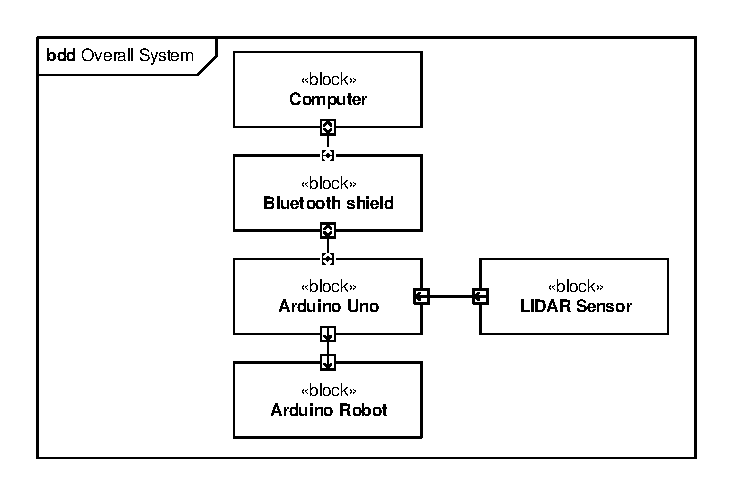
\includegraphics[width=0.7\textwidth]{billeder/OverallSystemDesign}
\caption{Overall System Design}
\label{fig:OSD}
\end{figure}
Each block in the system will now be discussed in greater detail. 

\subsubsection{Bluetooth shield}
The Bluetooth shield is an "ITEAD Wireless Bluetooth Shield Module Starter Kit For Arduino"\cite{BTshield}\cite{BTshield2}. The responsibility of the Bluetooth shield is to transfer data from the Arduino Uno to the Computer. The shield uses a HC-05 Serial Bluetooth module. Connecting to the shield is done by finding "H-C-2010-06-01" on the Computer and using the password: "1234". The settings for the serial bus is:
\begin{itemize}
\item Default baud rate: 9600
\item Data bits: 8
\item Stop bit: 1
\item No parity
\end{itemize}
This means that the Bluetooth connection can be seen as a simple uart connection between the robot and the computer. 

\subsubsection{LIDAR Sensor}
A LIDAR measurement consists of 90 packets with four range measurements in each. The packet length is 22 bytes and is organised as follows\cite{LIDAR}:
\begin{verbatim}
<start> <index> <speed_L> <speed_H> [Data 0] [Data 1] [Data 2] [Data 3]
 <checksum_L> <checksum_H>
\end{verbatim}
The $start$ code is 0xFA, $index$ goes from 0xA0 to 0xF9, $speed$ is the fixed point speed in RPM and $Data$ $N$ is the Nth reading. Each reading is four bytes in length and contains information about distance, signal strength and two flags. The data is comprised as follows:
\begin{verbatim}
<distance 7:0>  <"invalid data" flag> <"strength warning" flag> 
<distance 13:8> <signal strength 7:0> <signal strength 15:8>
\end{verbatim}
The LIDAR, also called Neato LIDAR can be seen in figure \ref{fig:NeatoLidar}.
\begin{figure}[H]
\centering
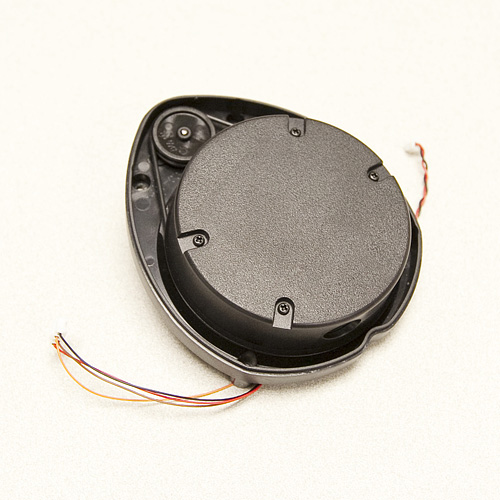
\includegraphics[scale=1]{billeder/NeatoLidar}
\caption{Neato LIDAR Sensor}
\label{fig:NeatoLidar}
\end{figure}
The LIDAR has four connects to the sensor part and two to the motor part. The motor connects are 3.3 Volt based with red being power and black being ground. The pinout for the sensor part is seen in table \ref{tab:lidars}.
\begin{table}[H]
\centering
\begin{tabular}{|l|l|}
\hline
Red & 3.3V \\ \hline
Brown & LDS\_RX \\ \hline
Orange & LDS\_TX \\ \hline
Black & GND \\ \hline
\end{tabular}
\caption{LIDAR Sensor Pinout}
\label{tab:lidars}
\end{table}
The motor is a simple DC-motor. But for a correct operation the Neato LIDAR must spin with more than 180 RPM and less than 350 RPM. The group found that a spin speed around 310 RPM gave the optimal sensor readings. This can be regulated using the speed information in the LIDAR data packets. The value in the speed bytes is formatted as RPM*64. So in order to get the RPM one must simply divide the value by 64. The group attained the optimal rotation speed, by regulating a PWM signal, on the motor. 

\subsubsection{Arduino Uno}
The Arduino Uno\cite{ArduinoUno} handles communication with the LIDAR Sensor and the Bluetooth shield.
\begin{figure}[H]
\centering
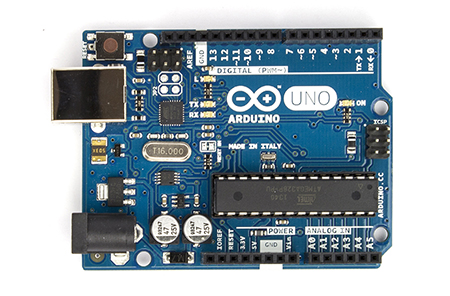
\includegraphics[scale=1]{billeder/ArduinoUno}
\caption{Arduino Uno}
\label{fig:ArduinoUno}
\end{figure}

The LIDAR data is streamed to the Arduino Uno contentiously with a baud rate on 115200. To handle the fast data rate the only hardware UART is used. The data is stored in a internal array for later retrieval.

Since there is only one hardware UART on the Arduino Uno, and both the LIDAR and the bluetooth shield needs one, a software serial port is created to handle the bluetooth communication. The Arduino Uno is listening for commands, on the bluetooth connection. A command is formatted as follows:
\begin{verbatim}
<command ID 1> <command ID 2> [Command parameters ] < 0x0A ('\n') >
\end{verbatim}
The following commands is handled by the Arduino Uno: 
\begin{tabbing}	
{LID}\={AR:}\\
\>{Comm}\={and1: <L> <D> <D/S/P/E> <\textbackslash n>} \\
\> \> D: Distance \\
\> \> S: Signal strength\\
\> \> P: Rotor speed\\
\> \> E: Error codes\\
\> return value:\\
\> \> {For D and S are the response: Array of 360 x 2 bytes big endian (the first is 0 deg)} \\ \> \> {(Distance in mm)} \\
\> \> {P are 2 byte value as big endian. Format are RPM*64} \\
\> \> {E is the same as D og S, excepted the array is only at size 360 x 1 byte} \\
\\
\> Command2: <U> <P> <\textbackslash n>\\
\> return value: \\
\> \> 1 byte \= formatted as: \\
\> \> \>{[0x00] if no LIDAR data is available.} \\
\> \> \>{[0x01] if LIDAR data is available.} 

\end{tabbing}	

If any other commands is received, they are sent to the Arduino Robot over the I2C interface. 

\subsubsection{Arduino Robot}
The robot platform used in this project is a Arduino robot\cite{ArduinoRobot}. The Arduino robot platform handles all movement commands. This is done with two boards, the motor board and the control board. 
Both boards are fitted with ATmega32u4 microcontrollers. The motor board has two motors, a power bank, various communication busses, ir sensors and an on/off switch along with the microcontroller. 
The motors are of the type DC. They are controlled with a pwm signal.\\
The Control board is fitted with a speaker, external memory, various communication busses, a compass and the possibility for a LCD display.\\
When equipped with the Arduino Uno, LIDAR Sensor and the Bluetooth shield, the platform can be seen in figure \ref{fig:fullplatform}.
\begin{figure}[H]
\centering
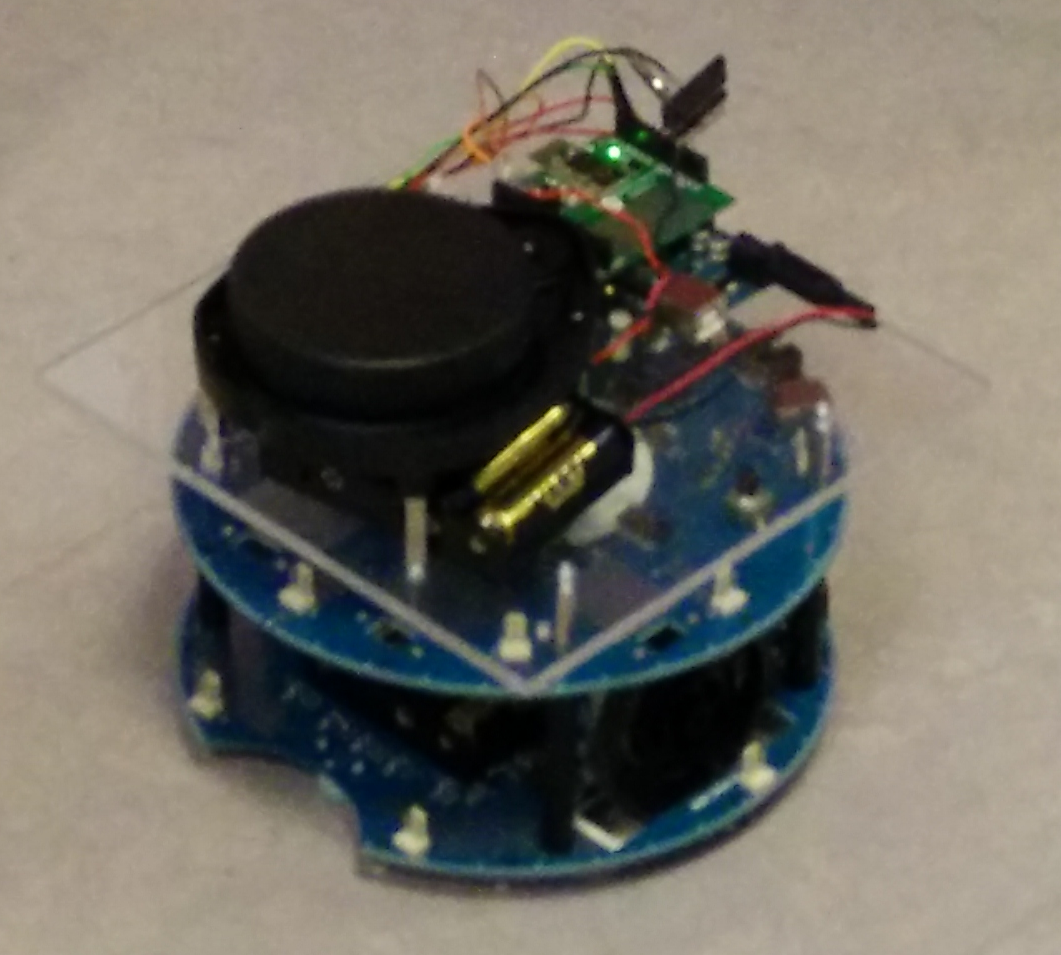
\includegraphics[width=0.6\textwidth]{billeder/fullplatform}
\caption{full platform}
\label{fig:fullplatform}
\end{figure}

The robot receives movement commands from the Arduino Uno and react on them. The Commands follows the same structure as the LIDAR commands. The Commands accepted by the robot is: 

\begin{tabbing}	
{Mot}\={or:}\\
\> {Comm}\={and: <M> <O> $[$Motor1$]$ $[$Motor2$]$ $[$Time$]$ <\textbackslash n> } \\
\> \> motor1 speed - 2 byte (-255 - 255) big endian \\
\> \> motor2 speed - 2 byte (-255 - 255) big endian\\
\> \> Time   - 2 byte big endian in ms.
\end{tabbing}	

\section{MATLAB Controller}
In this section the control actions done by the computer will be explained. The control program consists of the three sub components localisation, motion and planning. The aim of the control program is to first localize the robot. When this is achieved it must calculate a route to the desired goal, and move correctly to the goal. 

% Designandimp_Motion
\subsection{Motion}
The motion of the robot consists of two actions.
\begin{itemize}
\item Move forward 
\item Turn
\end{itemize}
Due to the lack of tachometers the robot needs an alternative way of figuring out how far it has moved or turned. The motion commands are therefore mainly based on time.

A general Move command is called by the command \textit{Move( socket, motor1, motor2, time )}, where socket is the bluetooth socket, motor1 is the speed of the right motor, motor2 is the speed of the left motor, both integer values in the range [-255:255], and time is the time in milliseconds.

\textbf{Move forward}\\
The Move forward command is called by the command \textit{[moved] = Move(obj, motor1, motor2, distance)}, where obj is the robot object, motor1 is the speed of the right motor, motor2 is the speed of the left motor, both integer values in the range [-255:255], and distance is the distance in cm. The moved parameter is the output of the Move forward command and contains the actual distance moved, based on LIDAR data.

This function consists of 2 parts. 
\begin{itemize}
\item Calculation of the time the robot must move to reach the desired distance.
\item Make sure that the robot does not bump into anything.
\end{itemize}
To find the time it takes for the robot to move, a measurement was made. The robot was placed behind a line, and different times were given to the function. The distance the robot travelled was then measured. In the end a function was fitted to the curve, and this function is the basic of the Move function.

\begin{figure}[H]
\centering
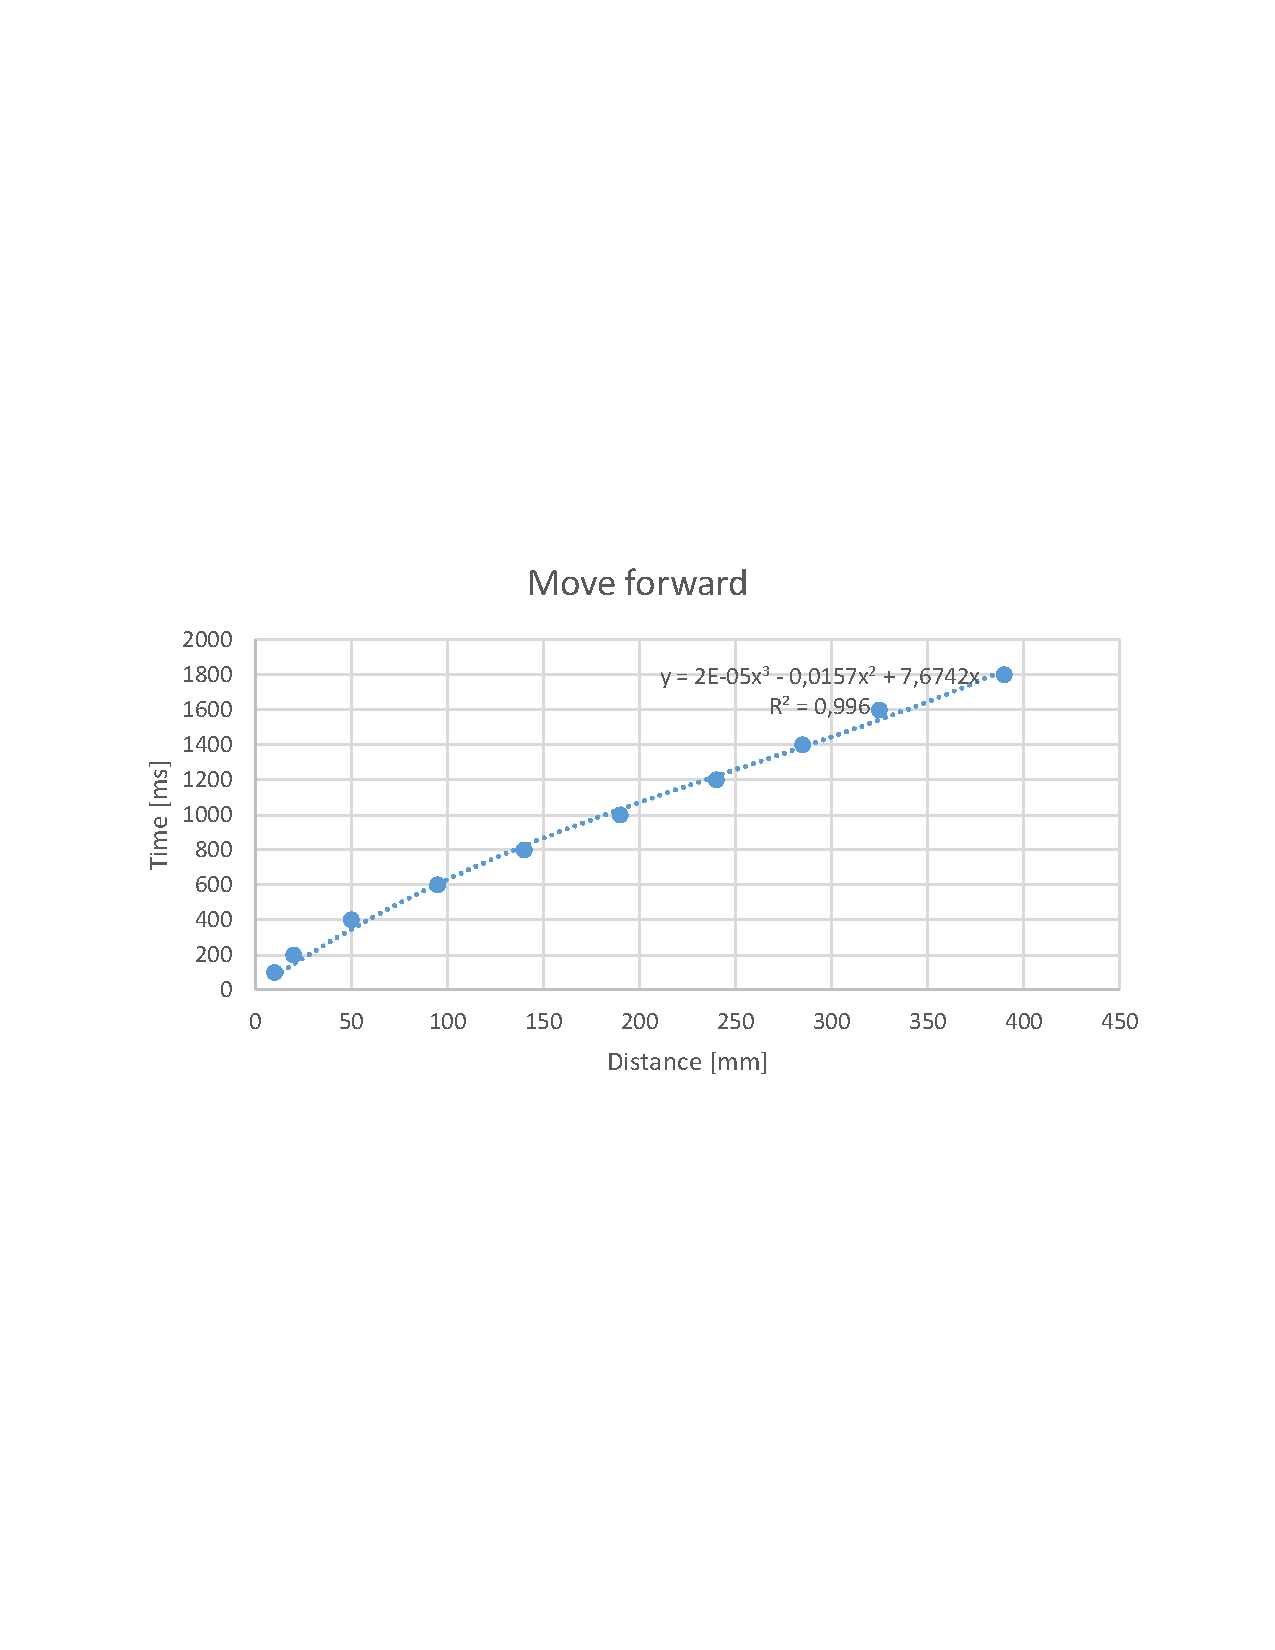
\includegraphics[width=0.8\textwidth]{billeder/MoveForwardGraph.pdf}
\caption{Measurement of Move forward}\label{MoveForwardGraph}
\end{figure} 

The main problem is that when the robot is using up battery, it does not move as far in the same given time as when it is fully charged. Therefore a measurement is made with the LIDAR before and after the movement to get a better fit of how far the robot actually moved. The measurement takes account of failing measurements, so that if the measurement straight ahead fails, it will use the nearest angle instead. The two distances is then calculated using trigonometry.
The difference between the two distances is the actual movement of the robot, and it is this value that is returned from the function.
The reason why LIDAR is not used directly to move a specific distance is the update rate of the LIDAR data. It is simply too slow. The function then calls the general Move command with the calculated time.

Despite the fact that the LIDAR has a slow update rate, it is used as a safe distance detection. If an object is detected in the area shown in figure \ref{MotionBumper}, the robot stops its movement and the function returns the moved distance. Due to the slow update rate of the LIDAR, the safe distance is relatively high. In the project, the forward safety distance is set to 250 mm. and the safety distance to each side is 200 mm.

\begin{figure}[H]
\centering
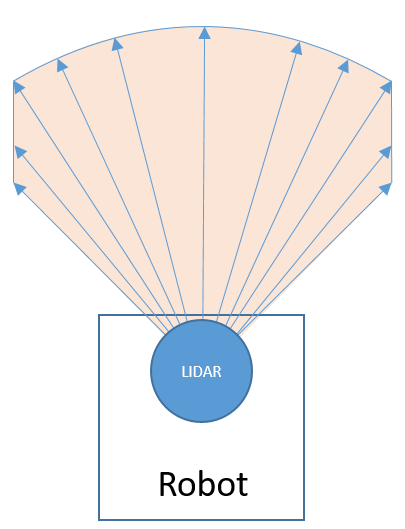
\includegraphics[scale=0.7]{billeder/MotionBumper.png}
\caption{Area of bump detection. The robot is facing up.}\label{MotionBumper}
\end{figure} 

\textbf{Turn}\\
The Turn command is called by the command \textit{Turn(obj, phi)}, where obj is the robot object and phi is the turning angle in degrees. The range of phi is [-180:180] with decimals accepted. This function calculates the time it will take for the robot to turn to the angle received, and calls the general Move function with one motor in reverse and the other in forward position. 
To get a way to calculate the time, a measurement similar to the on for the Move forward function was made. The robot was placed at a point and a mark was made where it had its 0 degrees. Then the general move function was called with different times and the angle the robot turned was measured. Figure \ref{TurnRightGraph} and \ref{TurnLeftGraph} shows the result of the measurements.

\begin{figure}[H]
\centering
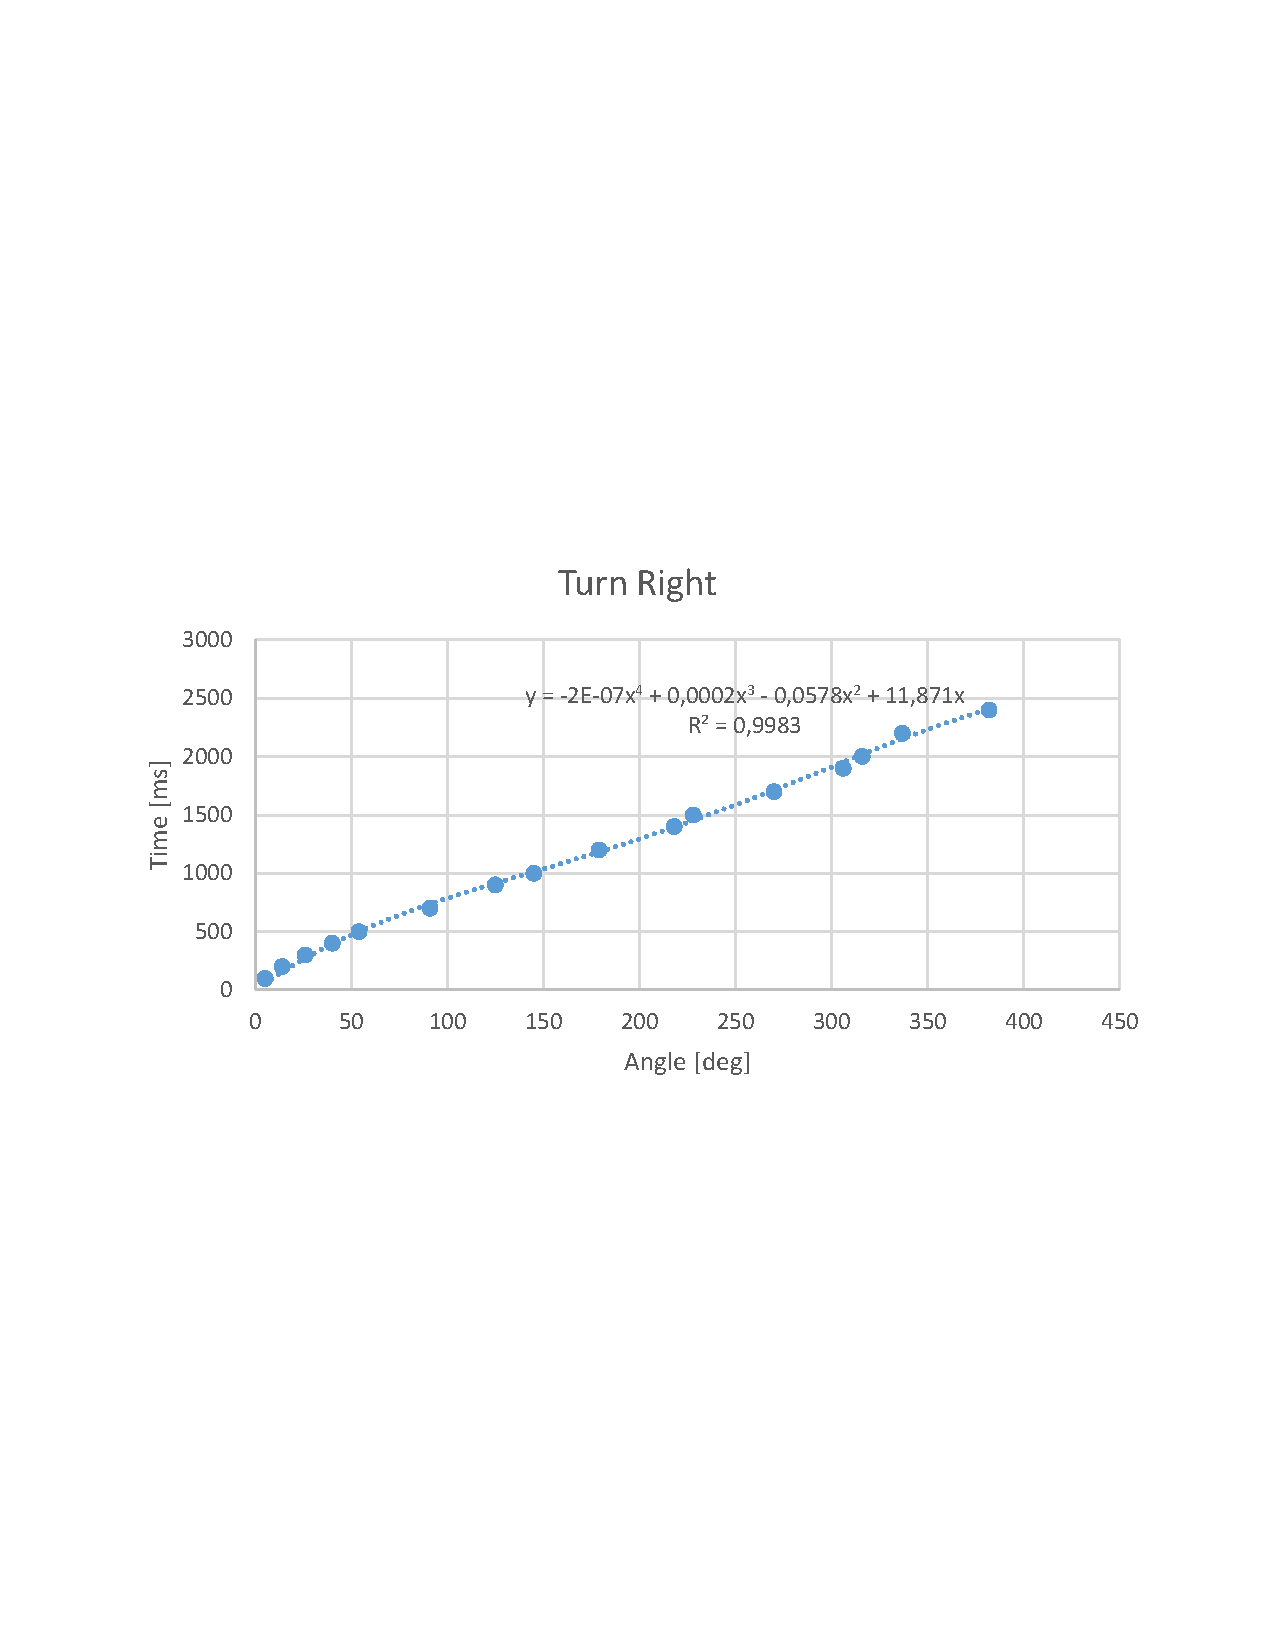
\includegraphics[width=0.8\textwidth]{billeder/TurnRightGraph.pdf}
\caption{Measurement of Turn right}\label{TurnRightGraph}
\end{figure} 
\begin{figure}[H]
\centering
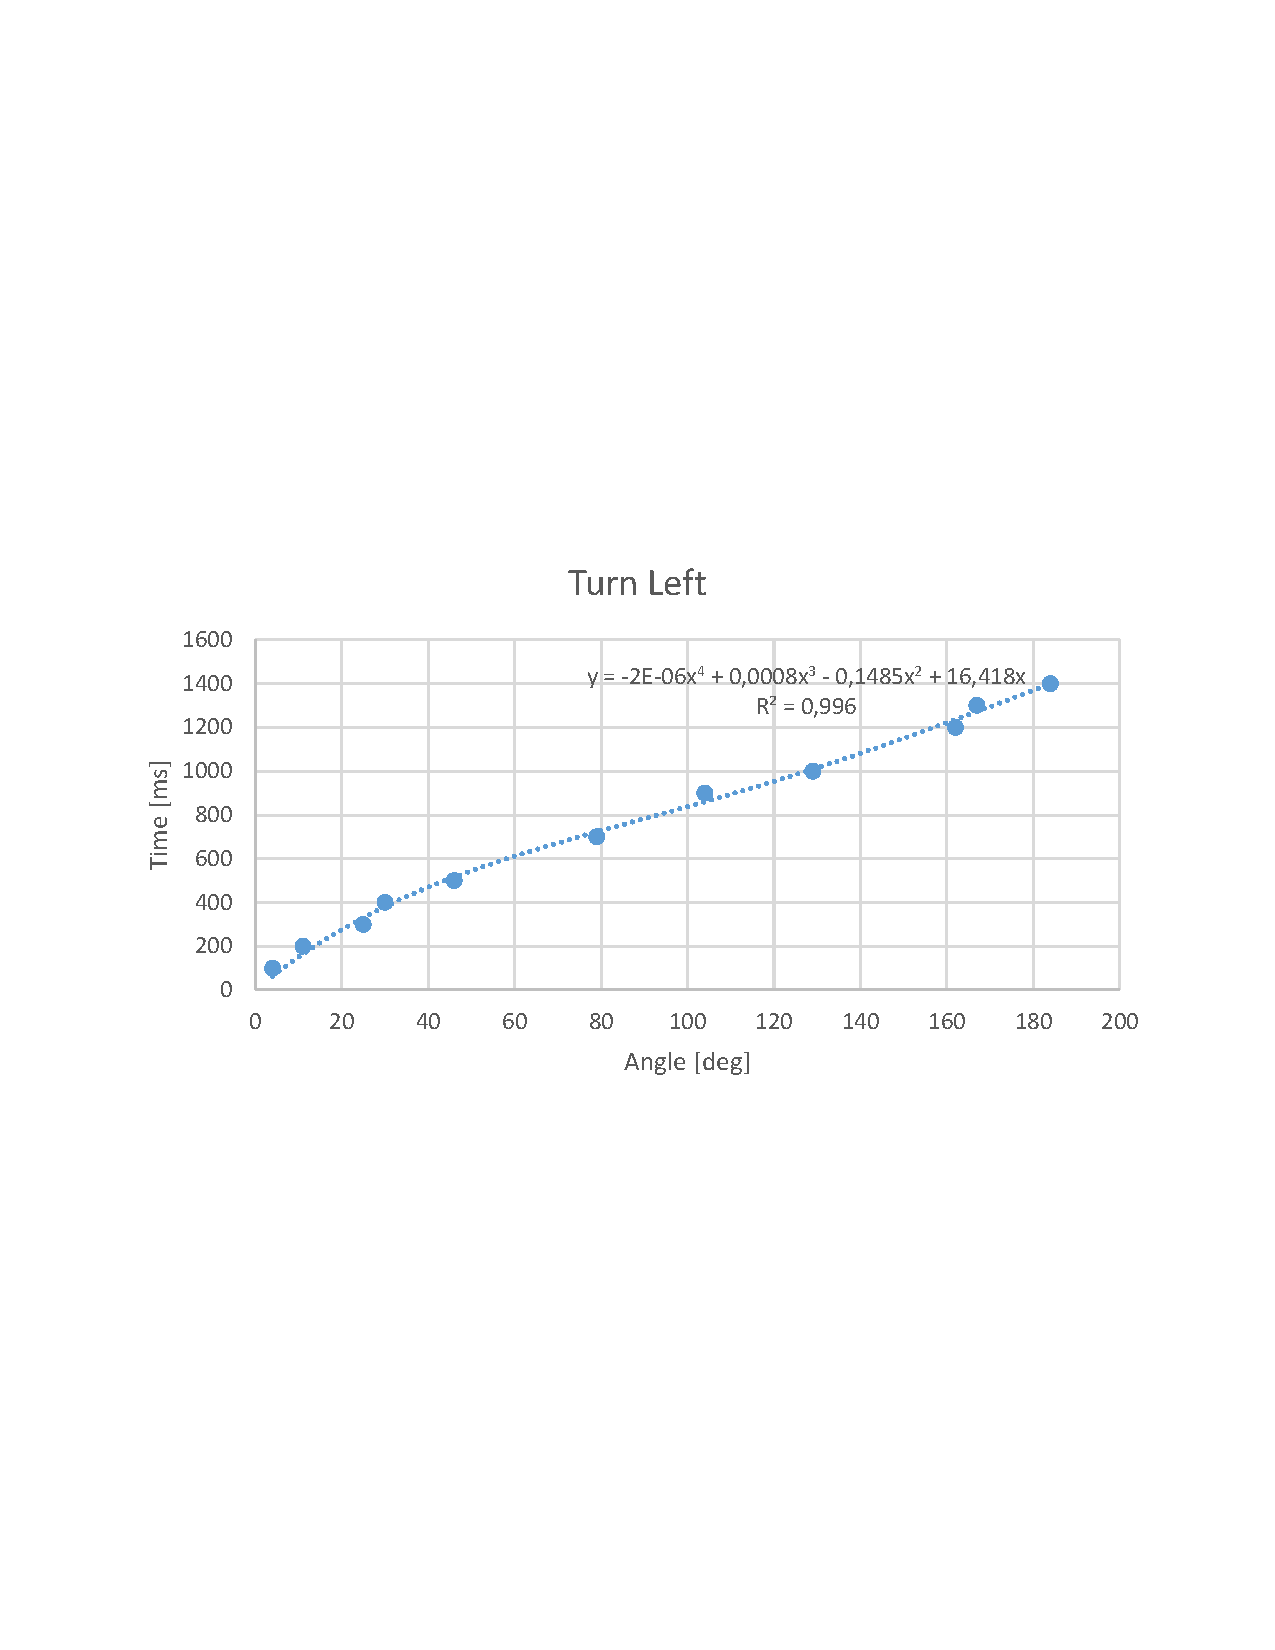
\includegraphics[width=0.8\textwidth]{billeder/TurnLeftGraph.pdf}
\caption{Measurement of Turn left}\label{TurnLeftGraph}
\end{figure} 

The same problem with the battery power arises in this function. Therefore a scanning is made by the LIDAR before the turn is performed. After the turn is made, the LIDAR scans again and the robot compares the two measurements by convolution. Then it starts to step one degree until a maximum in the convolution is found. This is then expected to be a more correct guess of the desired angle.


\subsection{Localisation Using Particle Filter}
In order to localize the robot a particle filter was used. The filter works by following a series of steps. 

\textbf{Step 1: Initialize the filter}\\
First 200 particles was created and given a random position and orientation on the map. In MATLAB this is simply a big 3x200 matrix with $[x, y, phi]$ for each of the 200 particles. 

\textbf{Step 2: Getting The Robot Measurement}\\
At this step we get the robot measurement. But even though all 360 measurements would give a very precise filter, the time it would take to calculate the particle distances in 360 degrease would be too long. In this project we have chosen to use 20 measurements, but less can in theory be used. The less measurements that are used in the filter, the bigger the risk of getting symmetric error locations. These locations will die over time, but for a system with too few measurements it can take quiet a while. 

The data from the robot is a series of distances and angels. If we plot this for our robot it can look like shown on figure \ref{RobotData}.

\begin{figure}[H]
\centering
\begin{subfigure}{.5\textwidth}
  \centering
  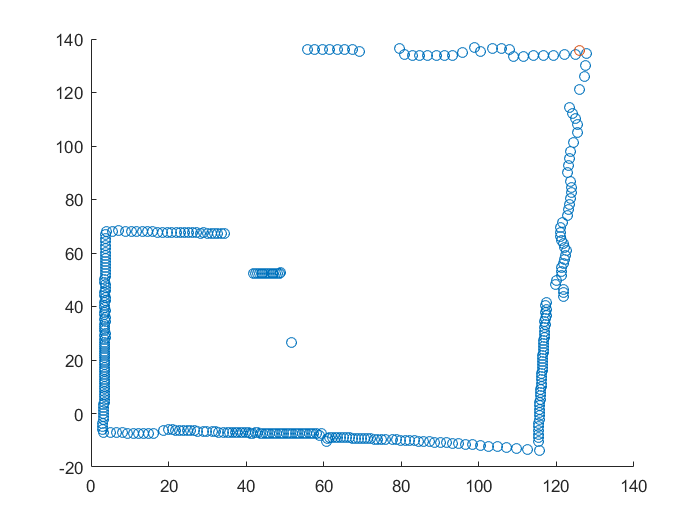
\includegraphics[width=1.2\linewidth]{billeder/SeeData.png}
  \label{ResultDriveFig1:sub1}
\end{subfigure}%
\begin{subfigure}{.5\textwidth}
  \centering
  \includegraphics[width=.6\linewidth]{billeder/Results/real3.png}
  \label{ResultDriveFig1:sub2}
\end{subfigure}
\caption{Robot LIDAR Data}
\label{RobotData}
\end{figure}

As seen on the figure there is a gap in the readings where the black pillar is at the top of the image. This is an area where the LIDAR is not able to read. This introduces another problem if we compare an error reading with a particle correct reading. This can give a good particle a bad probability later on.
To fix this we start taking only the good readings, and then take 20 measurements equally spaced from the set. We now have a set with 20 distances and what angle they where measured in. 

\textbf{Step 3: Getting The Particle Measurement}\\
Now the particles measurements at the same angles as the real robots measurements must be found. We have done this by a ray casting technique where we put a point at the particle position. Then we move the point a little bit in the beam direction and check if there is an obstacle. If this is not the case we move the point a little more. We continue this process till we hit an obstacle.\\
This is done for all particles in all measurement directions. When the algorithm is done the result is a 20x200 matrix containing all measurements for all particles. 

\textbf{Step 4: Calculating Particle probability}\\

By comparing each particles measurements to the real robots measurements the probability for how likely it is that the real robot have the same position and orientation as the particle is calculated. This is done using equation \ref{EQProb}. 

\begin{equation}
	Prob(P_{dis},R_{dis})= e^{-{\frac{(P_{dis_1} - R_{dis_1})^2}{2 \cdot Noise^2}}} \cdot e^{-{\frac{(P_{dis_2} - R_{dis_2})^2}{2 \cdot Noise^2}}} \cdot ... \cdot e^{-{\frac{(P_{dis_{20}} - R_{dis_{20}})^2}{2 \cdot Noise^2}}}
\label{EQProb}
\end{equation}

An important factor here is the noise that indicates how much a particle and the real robots measurements can differ, and still be a good fit. The noise must be set fairly high since we also want particles close to the true value to survive, and not just the ones on the true value. 

\textbf{Step 5: Finding The Best Fit}\\
At some point we need to decide where the robot is, according to the particle information. There are many approaches that can be used to decide this. Some look at the mean value, others look at clusters. In our implementation we took a simple approach and took the particle with the highest probability and selected as our guess on the robot location. 

\textbf{Step 6: Resample Or Reset}\\
Now it is time to do the resampling of the particles. This only make sense if there is atleast one good estimate since a resampling basically focuses the filter around the best guesses. If all guesses are bad, it will focus around random bad guesses. To counter effect this we made the filter restart and go back to step 1 if the best guess is under 10\% certainty. By doing this we force the filter to reset if it have no clue where the robot is. 

\textbf{Step 7: Move the robot}\\
In order to get a better estimate more information must be given to the filter. This can only be achieved if the robot moves. When the robot does not know where it is it can simply move randomly around. To simplify this behaviour we have made the robot move in the longest free direction it can see with the LIDAR. 

If the robot have a good guess on its location at this point it moves towards the next point in its movement plan. The movement plan is created the first time the robot get a guess on its location that is over 70\% certainty and is from that point on followed, unless the filter gets reset. The movement plan is the route calculated using A* from the robot location, found by the filter, to the desired goal. 

\textbf{Step 8: Updating the filter}\\
The filter is now updated by moving and turning all the particles the same amount as the real robot just did. In addition to the move, all particles are also moved and turn a little bit at random. This is to simulate the effect of the noise in the robot movement. After this step we go back to step 2 and continues from there in a never ending loop. 

After a few iterations the filter will collect all particles in a small cloud around the robot position. The width and height of the cloud is detriment by the movement noise, and the noise in particle probability equation. Finding good values for the noise model is critical for a well functioning filter. In our small project fixed values was used that was found over a process of trial and error.  Similar values could be found by creating a noise model for the robot and LIDAR. In more advanced implementations it is also common to use an adaptive approach changing the values on the fly. 
\subsubsection{Path Planning}
The path planning consist of two actions, finding a path with A\text{*} and then calculating coordinate targets in the map. 
A\text{*} uses a know map, an initial position, the goal and a cost map to plan out the path to the goal. 
The internal functionality of the A\text{*} function generates a heuristic map based on the goal and the know map. The implementation of A\text{*} is based upon the implementation from the Artificial Intelligence in Robotics Udacity course\citep{AIROK}.\\
The output of the A\text{*} is a path and a policy vector. The policy vector is used to calculate some coordinate targets which are used as targets when the robot moves towards the goal. An example of a plan can be seen in figure \ref{fig:exastar} where start is [ 1 1 ] and the goal is [ 6 5 ]. For a real world example see the results section.
\begin{figure}[H]
\centering
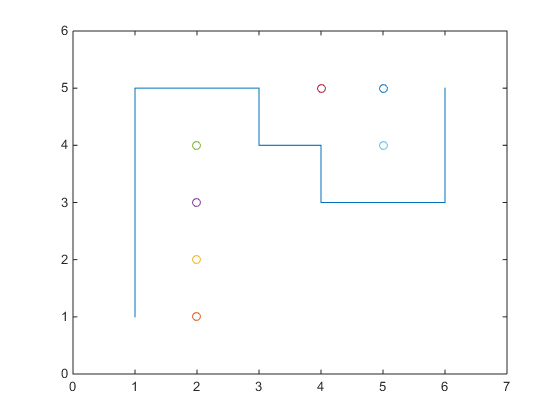
\includegraphics[width=0.5\textwidth]{billeder/exampleastar}
\caption{Example of A star plan}
\label{fig:exastar}
\end{figure}
 
%------------------------------------------------